\documentclass[tikz,border=10pt]{standalone}
\usepackage{tikz}
\usetikzlibrary{angles,quotes,calc}
\usepackage{tkz-euclide} %for right angle marker

\begin{document}
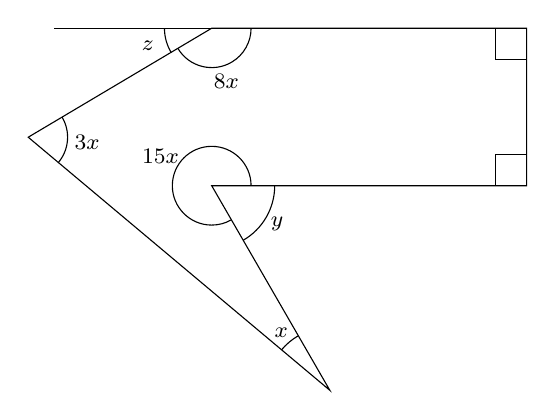
\begin{tikzpicture}[scale = 1]
    % Initial point
    \coordinate (A) at (0,0);
    % Draw octagon
    \draw (A) -- ++(0:4cm) coordinate(B) -- ++(-90:2cm) coordinate (C) -- ++(180:4cm)  coordinate (D) -- ++(300:3cm) coordinate (E) -- ++(140:5cm) coordinate (F) -- cycle;

    % Draw extended line
    \draw (A) -- (-2,0) coordinate (G);
    
    % Draw the angle between lines
    \pic [draw, "\footnotesize $z$ ", angle eccentricity=1.4, angle radius=0.6cm] {angle = G--A--F};
    \pic [draw, "\footnotesize $8x$", angle eccentricity=1.4, angle radius=0.5cm] {angle = F--A--B};
    \pic [draw, "\footnotesize $x$", angle eccentricity=1.2, angle radius=0.8cm] {angle = D--E--F};
    \pic [draw, "\footnotesize $3x$", angle eccentricity=1.5, angle radius=0.5cm] {angle = E--F--A};
    \pic [draw, "\footnotesize $15x$", angle eccentricity=1.5, angle radius=0.5cm] {angle = C--D--E};
    \pic [draw, "\footnotesize $y$", angle eccentricity=1.2, angle radius=0.8cm] {angle = E--D--C};

    %marking right angles
    \tkzMarkRightAngle[size=.4](A,B,C);
    \tkzMarkRightAngle[size=.4](B,C,D);
    
    
\end{tikzpicture}
\end{document}

